\section{Elements}

\subsection{Blocks}

\begin{frame}{Definition}
	The definition below is from \cite{angluin1980local}.

	\begin{definition}
		Here is a definition block.
	\end{definition}
\end{frame}

\begin{frame}{Theorem}
	The following is proved in \cite[pp.~74--75]{yamashita1996computing1}.

	\begin{theorem}
		Here is a theorem block.
	\end{theorem}
\end{frame}

\begin{frame}{Alert}
	If you want to alert something, \alert{just do it}.

	\begin{alertblock}{Notice}
		I can eat glass. It does not hurt me.
	\end{alertblock}
\end{frame}

\begin{frame}{You Can Also Define by Yourself}
	\begin{block}{Conjecture}
		An \((x, bx)\)-biregular graph \(G = (U \cup V, E)\) is the union of \(b\) edge-disjoint bipartite \(x\)-regular subgraphs.
	\end{block}
\end{frame}

\subsection{List Environments}

\begin{frame}{Unordered/Order List}
	\begin{columns}
		\begin{column}{0.5\textwidth}
			What a panda cub can bite:
			\begin{itemize}
				\item Bamboos
				\item Cookies
				\item Glass, of course
			\end{itemize}
		\end{column}

		\begin{column}{0.5\textwidth}
			What you have to do next:
			\begin{enumerate}
				\item Eat
				\item Pray
				\item Love
			\end{enumerate}
		\end{column}
	\end{columns}
\end{frame}

\begin{frame}{List With Item Labels}
	\begin{description}
		\item[Morgan] An American financier and banker
		\item[Bach] A German composer and musician
		\item[Naipaul] A Trinidad and Tobago-born British writer
	\end{description}
\end{frame}

\subsection{Illustrations}

\begin{frame}{Figures}
	\begin{figure}[ht]
		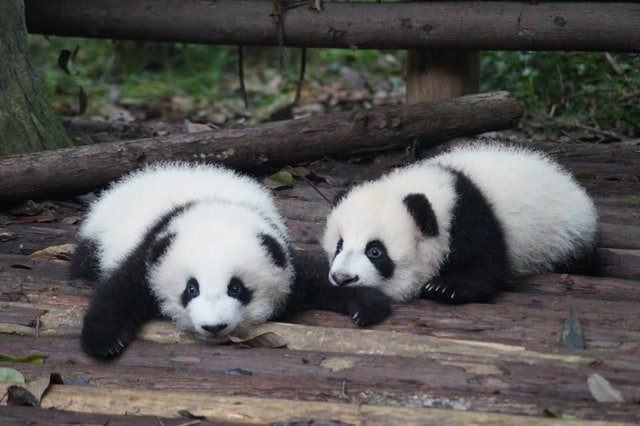
\includegraphics[width = 0.5\textwidth]{Figures/Panda_Cubs.jpg}
		\caption{(\href{https://unsplash.com/photos/4EajIuUxgAQ}{Photo} by \href{https://unsplash.com/@millerthachiller}{Pascal M\"{u}ller} on \href{https://unsplash.com/}{Unsplash})}
	\end{figure}
\end{frame}

\begin{frame}{Tables}
	\begin{table}[ht]
		\centering
		%!TEX root = ../Main.tex

\begin{tabular}{c || cccc}
	\textbf{Degree Tree \(D_i\) (Key)} & \(D_1\) & \(D_2\) & \(\dots\) & \(D_{\kappa}\) \\
	\hline
	\textbf{Degree Tree Class \(V_{D_i}\) (Value)} & \(V_{D_1}\) & \(V_{D_2}\) & \(\dots\) & \(V_{D_{\kappa}}\) \\
\end{tabular}

		\caption{Table 1}
	\end{table}

	\begin{table}[ht]
		\centering
		%!TEX root = ../Main.tex

\begin{tabular}{||c c c c||}
	\hline
	ID & Age & Salary & Panda \\
	\hline\hline
	1 & 11 & 11111 & 11 \\
	\hline
	2 & 7 & 78 & 0 \\
	\hline
	3 & 121 & 0 & 302 \\
	\hline
	4 & 43 & 18744 & 1 \\
	\hline
	5 & 88 & -342 & 6344 \\
	\hline
\end{tabular}

		\caption{Table 2}
	\end{table}
\end{frame}